
\begin{figure}
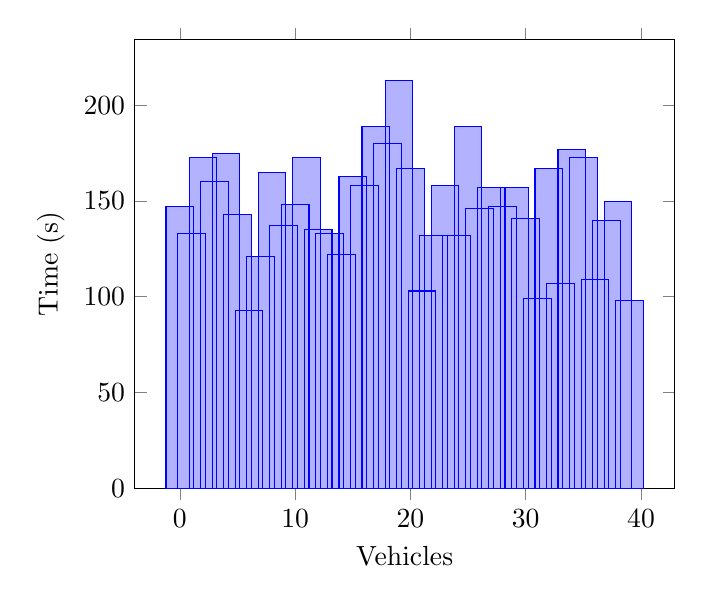
\begin{tikzpicture}
\begin{axis}[
legend style={anchor=west},
xlabel=Vehicles,
ylabel=Time (s),
ymin=0,
ybar,
]
\addplot coordinates {
(0, 147)
(1, 133)
(2, 173)
(3, 160)
(4, 175)
(5, 143)
(6, 93)
(7, 121)
(8, 165)
(9, 137)
(10, 148)
(11, 173)
(12, 135)
(13, 133)
(14, 122)
(15, 163)
(16, 158)
(17, 189)
(18, 180)
(19, 213)
(20, 167)
(21, 103)
(22, 132)
(23, 158)
(24, 132)
(25, 189)
(26, 146)
(27, 157)
(28, 147)
(29, 157)
(30, 141)
(31, 99)
(32, 167)
(33, 107)
(34, 177)
(35, 173)
(36, 109)
(37, 140)
(38, 150)
(39, 98)
};

\end{axis}
\end{tikzpicture}
\label{tik:100:97}
\caption{100 percent diving with GSC on route $97$}
\end{figure}
